\documentclass{article}
\usepackage[usenames,dvipsnames]{color,xcolor}
\usepackage{listings}
\usepackage{hyperref}
\usepackage{amsmath,amsthm,amssymb,mathtools,fancyhdr,tcolorbox,cancel,pgfplots,tikz}
\usetikzlibrary{intersections}
\usepackage[right=3.75cm,left=3.75cm,top=4cm,bottom=4cm]{geometry}

\theoremstyle{definition}
\newtheorem{definition}{Definition}
\newtheorem{ub}{Aufgabe}
\newtheorem*{lo*}{Lösung}
\newtheorem*{lem*}{Lemma}

\begin{document}
	
	\thispagestyle{plain}
	\begin{minipage}{5cm}
		
\includegraphics[width=5cm]{logo}\\
		\centering
		Fakultät für Mathematik
	\end{minipage}
	\hfill
	\begin{minipage}{7cm}
		\baselineskip=.4cm
		Arman Sadeghi Rad\\
		Matrikelnummer 12223560 \\
		Einführung in das mathematische Arbeiten \\
		Wintersemester 2022/2023
	\end{minipage}\\[1mm]
	\hrule height2pt \vskip1mm
	\noindent
	Übungsblatt 5A
	\hrule height2pt \vskip1mm

\begin{ub}
	\begin{lo*}[1]
		\[ 
		a < b \xRightarrow[]{\text{O1}} 0 = a + (-a) < b + (-a) \Rightarrow 0 < b-a.
		 \]
		Ebenso gilt $ 0 < d - c $. Danach gemäß O1:
		\[ 
		(b+d) - (a+c) = b-a + d-c > d-c > 0 \Rightarrow 
		(b+d) - (a+c) > 0 \Rightarrow
		\boxed{a+c < b+d}.
		 \]
	\end{lo*}
	\begin{lo*}[2]
		\[ 
		a<b \xRightarrow[]{\text{6.3.2(i)}} b-a > 0, c > 0 \xRightarrow[]{\text{O2}} (b-a)c = bc - ac > 0. \tag{1}\label{1.2.1}
		 \]
		\[ 
		c<d \xRightarrow[]{\text{6.3.2(i)}} d-c > 0, b > 0 \xRightarrow[]{\text{O2}} (d-c)b = bd-bc > 0.
		\tag{2}\label{1.2.2}
		 \]
		nach L\"osung von (1) und die Ungleichungen von \ref{1.2.1} und \ref{1.2.2} gilt
		\[ 
		bc - ac + bd - bc = bd - ac > 0 + 0 = 0 \Rightarrow ac < bd.
		 \]
	\end{lo*}
\end{ub}
\begin{ub}
	\begin{lo*}[1]
		Beginnen wir den Beweis mit einem Lemma. 
		\begin{lem*}\label{lemm}
			Wenn \( a > b > 0 \) und \( c \geq d > 0 \) dann \( ac > bd \) und \( ac = bd \) ist unmöglich.
			\begin{proof}[Beweis]
				Angenommen, es gibt $ a,b,c $ und $ d $ mit solchen Ungleichheiten, dass $ ac = bd $.
				dann gilt \( c = \frac{bd}{a} = \frac{b}{a}d \). Aus $ b^{-1} > a^{-1} $ kann man folgern, dass $ 1 = b^{-1}b > ba^{-1} = \frac{b}{a} $.
				Aber $ d > 0 $ und daher $ c = \frac{b}{a}d < d $. Und es ist ein Widerspruch zu der Annahme, dass $ c \geq d $.
			\end{proof} 
		\end{lem*}
		\noindent $ x \geq a > 1 \Rightarrow x > 1 $ und $ x \geq a $. Daher $ x^2 > a $. Die Aussage 
		$ x^n > a $ kann man durch vollständige Induktion beweisen. Sei $ x^2 > a $ die Annahme und
		$ x^n > a $ die Behauptung, aus den Ungleichheiten $ x^n > a $ und $ x > 1 $ und Lemma, kann man folgern, dass auch $ x^{n+1} > a $ gilt. und die Aussage wird bewiesen.
	\end{lo*}
	\begin{lo*}[2]
		\[ 
		b < 1 \xRightarrow[]{\text{Aufgabe 1.2}} b^2 < 1 \Rightarrow \ldots \Rightarrow 
		b^{n-1} < 1 \Rightarrow 1 - b^{n-1} > 0 \xRightarrow[\text{O2}]{b>0}
		\Rightarrow b - b^n > 0 \Rightarrow b^n < b.
		 \]
	\end{lo*}
\end{ub}
\begin{ub}
	\begin{lo*}[1]
		\begin{proof}[b > a]
			\[ 
			\frac{a+b+|a-b|}{2} = \frac{a+b + b -a}{2} = b = \max\{a,b\}.
			 \]
		\end{proof}
		\begin{proof}[a > b]
			\[ 
			\frac{a+b+|a-b|}{2} = \frac{a+b + a -b}{2} = a = \max\{a,b\}.
			 \]
		\end{proof}
		\begin{proof}[a=b]
			\[ 
			\frac{a+a}{2} = \frac{a+b + a -b}{2} = a = \max\{a,b\} = b.
			\]
		\end{proof}
	\end{lo*}
\end{ub}
\begin{ub}
	Angenommen, dass $ \sup\limits_{m \in \mathbb{N}}A_m $ geringer als $ 1 $ ist. Dann gibt es eine positive rationale Zahl $ \beta $, die $ \sup\limits_{m \in \mathbb{N}}A_m = 1 - \beta $. Dann $ 1 - \frac{\beta}{2} $ ist auch eine rationale Zahl die im Intervall $ (0,1) $ liegt. Nehmen wir an, dass
	$ q_k = 1 - \frac{\beta}{2} $. Dann $ q_k \in A_k $ und $ \sup\limits_{m \in \mathbb{N}}A_m $ könnte nicht $ 1 - \beta $ sein, weil $ 1-\frac{\beta}{2} > 1- \beta $. Ähnlicherweise ist auch die Aussage $ \inf\limits_{m \in \mathbb{N}}A_m = 0 $ richtig.
\end{ub}
\begin{ub}
	\begin{lo*}[1]
		\[ 
		\begin{array}{ccc}
			5 - 3x  \leq 2x+1 & \Rightarrow & x \geq \frac{4}{5} \\
			2x+1 \leq 3x-7 & \Rightarrow & x \geq 8
		\end{array} \Rightarrow x \geq 8
		 \]
	\end{lo*}
	\begin{lo*}[2]
	\[ 
	\begin{array}{cccc}
		2x-3 = 4x+9 & \Rightarrow & 2x = -12 & \Rightarrow x = -6 \\
		3 - 2x = 4x+9 & \Rightarrow & 6x = -6 & \Rightarrow x = -1
	\end{array}
	 \]
	\end{lo*}
	\begin{lo*}[3]
		\( 
		f(x) = 4x^2 - 9x - 5 \Rightarrow r_1 = \frac{9-\sqrt{161}}{8}, r_2 = \frac{9 + \sqrt{161}}{8}.
		 \)
		\begin{center}
					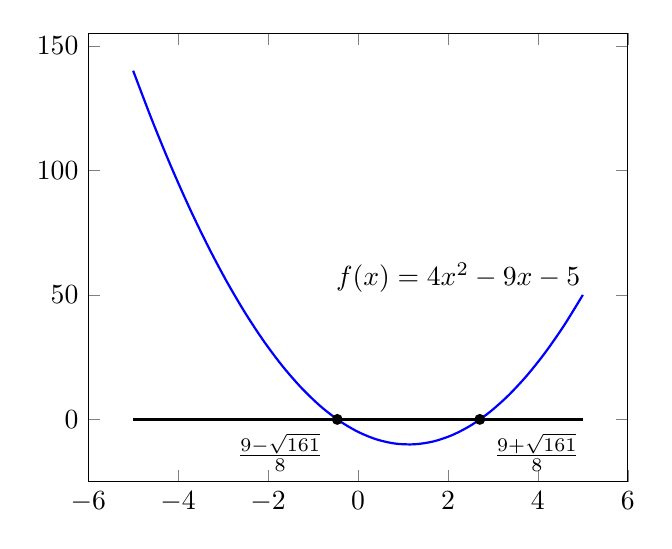
\begin{tikzpicture}		
				\begin{axis}
					\addplot[
					smooth,
					thick,
					blue,
					name path global = h1
					] {4*(x)^2 - 9*x - 5} node[above left,inner sep=.6pt,black,pos=1] {$f(x) = 4x^2 - 9x - 5$} ;
					\addplot[
					thick,
					black,
					name path global = h2
					]{0};
					\fill [name intersections={of=h1 and h2,by={E1,E2}}] (E2)
					node[circle,fill,inner sep=1.4pt,label=below right:$\frac{9 + \sqrt{161}}{8}$]{};
					\fill [name intersections={of=h1 and h2,by={E1,E2}}] (E1)
					node[circle,fill,inner sep=1.4pt,label=below left:$\frac{9 - \sqrt{161}}{8}$]{};
				\end{axis}
			\end{tikzpicture}
		\end{center}
	Daher muss $ x $ im Intervall $ [r_1 , r_2] $ sein.
	\end{lo*}
	\begin{lo*}[4]
		\[
		\frac{5+x}{5-x} - 2 = \frac{3x-5}{5-x} \leq 0. \Rightarrow x > 5 \,\, \text{oder} \,\,
		x \leq \frac{5}{3}.  
		 \]
		 Dann ist die Lösungsmenge, die Menge 
		 $ (-\infty , \frac{5}{3}] \cup (5,\infty) $.
	\end{lo*}
	\begin{lo*}[5]
		\[ 
		\begin{array}{ccl}
			\frac{2x-1}{3-2x} < \frac{1}{2} & \Rightarrow & x \in (-\infty , \frac{5}{6}) \cup (\frac{3}{2} , +\infty) \\
			\frac{2x-1}{3-2x} > \frac{1}{3} & \Rightarrow & x \in \mathbb{R} \setminus \{\frac{3}{2}\}
		\end{array} \Rightarrow x \in (-\infty , \frac{5}{6}) \cup (\frac{3}{2} , +\infty)
		 \]
	\end{lo*}
	\begin{lo*}[6]
		\[ 
		\begin{array}{ccl}
			x+4 \leq 6 & \Rightarrow & x \leq 2 \\
			5x+4 \geq 6 & \Rightarrow & x \geq \frac{2}{5}
		\end{array} \Rightarrow x \in [\frac{2}{5},2]
		 \]
	\end{lo*}
	\begin{lo*}[7]
		\begin{align*}
			\begin{array}{ccl}
				3x+4 \leq x+8 & \xRightarrow{x \geq -\frac{4}{3}} & x \leq 2 \\
				-3x-4 \leq x+8 & \xRightarrow[]{-8 \leq x < -\frac{4}{3}} & x \geq -4 \\
				3x+4 \geq x+8 & \xRightarrow[]{x < -8} & x > 2
			\end{array} & : ((-\infty , 2] \cap (-\frac{4}{3},+\infty)) \cup 
		([-8,-\frac{4}{3}) \cap [-4,+\infty)) \cup (-\infty , -8) \cap (2,+\infty) \\
		& = [-4,2]\setminus {-\frac{4}{3}}
		\end{align*}
	\end{lo*}
\end{ub}
\begin{ub}
	\begin{lo*}
		\begin{enumerate}
			\item 
			\( |ab| = -ab \)
			\begin{align*}
				(a+b)^2 \geq 0 & \iff a^2 + b^2 + 2ab \geq 0 \\
				& \iff a^2 + b^2 \geq -2ab \\
				& \iff \frac{a^2 + b^2}{2} \geq -ab = |ab|. 
			\end{align*}
			\item $ |ab| = ab $
			\begin{align*}
				(a-b)^2 \geq 0 & \iff a^2 + b^2 + 2ab \geq 0 \\
				& \iff a^2 + b^2 \geq 2ab \\
				& \iff \frac{a^2 + b^2}{2} \geq ab = |ab|. 
			\end{align*} 
		\end{enumerate}
	\end{lo*}
\end{ub}
\begin{ub}
	\begin{lo*}
		Die Operation ist Wohldefiniert genau dann wenn $ (a,b),(a',b'),(a'',b'') \in \mathbb{N} \times \mathbb{N} $
		\[ 
		(a,b) \sim (a',b') \Rightarrow [(a,b)] \otimes [(a'',b'')] \sim [(a',b')] \otimes [(a'',b'')].
		 \]
		\begin{align*}
			(a,b) \sim (a',b') & \Longrightarrow a + b' = a' + b \xRightarrow[\times a'']{\times b''}
			\left\{
			\begin{array}{ccc}
				ab'' + b'b'' = a'b'' + bb'' \\
				aa'' + b'a'' = a'a'' + ba''
			\end{array}
			\right. \\
			& \Longrightarrow (aa'' + b'a'') + (a'b'' + bb'')
			= (a'a'' + ba'') + (ab'' + b'b'') \\
			& \Longrightarrow [(a,b)] \otimes [(a'',b'')] \sim [(a',b')] \otimes [(a'',b'')]
		\end{align*}
	\end{lo*}
\end{ub}
\begin{ub}
	\begin{lo*}[1]
		\[ 
		a < b \xRightarrow[a \leq a]{\text{Aufgaben 1.2 und \hyperref[lemm]{Lemma}}}
		a^2 < ab
		 \]
		 \[ 
		 a < b \xRightarrow[b \leq b]{\text{Aufgaben 1.2 und \hyperref[lemm]{Lemma}}}
		 ab < b^2.
		 \]
		 Daher $ a^2 < ab < b^2 $.
	\end{lo*}
	\begin{lo*}[2]
		\[ 
		a < b \xRightarrow[]{\text{O1}} a + a < a + b \Rightarrow 2a < a+b 
		\Rightarrow a + b - 2a > 0 \xRightarrow[\text{O2}]{2^{-1} > 0} 
		 0 < \frac{a+b}{2} - a \Rightarrow \frac{a+b}{2} > a.
		 \]
		\[ 
		a < b \xRightarrow[]{\text{O2}} a + b < b + b \Rightarrow a + b < 2b 
		\Rightarrow a + b - 2b < 0 \xRightarrow[O2]{2^{-1} > 0} \frac{a+b}{2} - b < 0
		\Rightarrow \frac{a+b}{2} < b.
		 \]
		Daher $ a < \frac{a+b}{2} < b $.
	\end{lo*}
\end{ub}
\end{document}